% topic1.tex -- Module 7 Topic 1: Electromagnetic spectrum, Q1-18.
\firsttopictitle{Topic 1 - Electromagnetic Spectrum}

% ---- Q1 (Maxwell's prediction of the speed)
\begin{quizq}{}
Maxwell predicted the speed of electromagnetic waves. What did he use to calculate this speed?
\opts{The constants $\mu_0$ and $\varepsilon_0$, from experiments on magnetism and electricity}
  {Fizeau's measurement of the speed of light}{The frequency of light emitted by hot objects}
  {The photoelectric effect}
\end{quizq}

% ---- Q2 (structure of an EM wave)
\Needspace{14\baselineskip}
\begin{quizq}{}
Which statement about electromagnetic waves is correct?
\opts{The electric and magnetic fields oscillate parallel to each other.}
  {They need a medium, such as air, to travel through.}
  {In a vacuum, high-frequency waves travel faster than low-frequency waves.}
  {The electric and magnetic fields oscillate at right angles to each other and to the direction of
   travel.}
\end{quizq}

% ---- Q3 (production of EM waves)
\Needspace{12\baselineskip}
\begin{quizq}{}
Which of the following produces electromagnetic waves?
\opts{A charge at rest}{A charge moving at a constant velocity}{An oscillating charge}
  {A steady current in a straight wire}
\end{quizq}

% ---- Q4 (c from mu0 and epsilon0)
\Needspace{12\baselineskip}
\begin{quizq}{}
Given $\mu_0 = 4\pi \times 10^{-7}\,\si{N.A^{-2}}$ and $\varepsilon_0 = \qty{8.854e-12}{C^2.N^{-1}.m^{-2}}$,
what value does $\dfrac{1}{\sqrt{\mu_0\varepsilon_0}}$ give?
\opts{\num{1.1e-17}}{\num{3.3e-9}}{\num{9.0e16}}{\num{3.0e8}}
\end{quizq}

% ---- Q5 (Fizeau's toothed wheel)
\Needspace{16\baselineskip}
\begin{quizq}{}
In Fizeau's experiment, light passed through a gap between the teeth of a rotating wheel, travelled to a
mirror \qty{8633}{m} away and back, and was first blocked by the next tooth when the wheel turned at
12.6 revolutions per second. The wheel had 720 teeth, so the light's round trip took the time for the
wheel to turn half the distance from one tooth to the next. What value did this give for the speed of
light?
\opts{\qty{4.4e5}{m.s^{-1}}}{\qty{1.6e8}{m.s^{-1}}}{\qty{3.1e8}{m.s^{-1}}}{\qty{6.3e8}{m.s^{-1}}}
\end{quizq}

% ---- Q6 (types of spectra)
\Needspace{22\baselineskip}
\begin{quizq}{}
Which row of the table correctly matches each light source with the type of spectrum it produces?
\begin{center}
  \renewcommand\arraystretch{1.7}
  \begin{tabular}{@{}p{10mm}|>{\centering\arraybackslash}p{35mm}|>{\centering\arraybackslash}p{35mm}|>{\centering\arraybackslash}p{40mm}|}
    \cline{2-4}
    & \textit{Hydrogen discharge tube} & \textit{Incandescent filament} & \textit{Sunlight}\\ \cline{2-4}
    A. & Continuous & Emission lines & Absorption lines\\ \cline{2-4}
    B. & Emission lines & Continuous & Absorption lines\\ \cline{2-4}
    C. & Absorption lines & Continuous & Emission lines\\ \cline{2-4}
    D. & Emission lines & Absorption lines & Continuous\\ \cline{2-4}
  \end{tabular}
\end{center}
\end{quizq}

% ---- Q7 (how absorption lines form)
\Needspace{15\baselineskip}
\begin{quizq}{}
How are the dark lines in the spectrum of a star produced?
\opts{The star emits no light at all at those wavelengths, because its core is too cool.}
  {Cooler gas in the outer layers of the star absorbs particular wavelengths from the continuous
   spectrum emitted below it.}
  {Earth's atmosphere absorbs all the light at those wavelengths.}
  {Light at those wavelengths is slowed down by the star's gravity.}
\end{quizq}

% ---- Q8 (identifying elements from lines)
% Star lines at 1.0, 1.6, 2.5, 3.4, 4.3 (cm along the strip): X has 1.0, 2.5, 4.3; Z has 1.6, 3.4;
% Y has 0.6, 2.9, 3.9 (not in the star).
\Needspace{30\baselineskip}
\begin{quizq}{}
The diagram shows the absorption lines in the spectrum of a star, and the emission lines of three
elements, X, Y and Z, measured in a laboratory. All four spectra use the same wavelength scale.
\begin{center}
  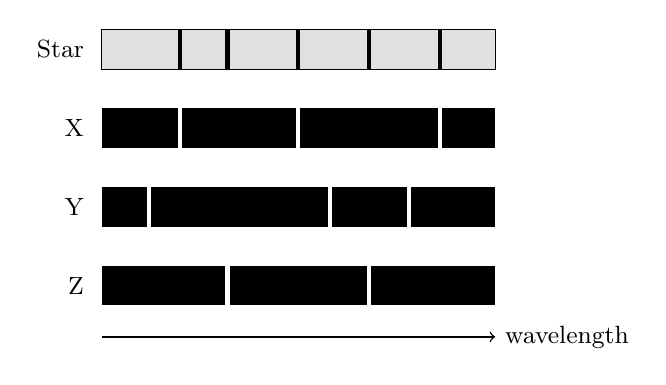
\begin{tikzpicture}
    \foreach \y/\l in {3/Star, 2/X, 1/Y, 0/Z} {\node[left, font=\small] at (-0.1,\y+0.25) {\l};}
    \fill[black!12] (0,3) rectangle (5,3.5); \draw (0,3) rectangle (5,3.5);
    \foreach \x in {1.0,1.6,2.5,3.4,4.3} \draw[line width=1.5pt] (\x,3) -- (\x,3.5);
    \foreach \y/\lines in {2/{1.0,2.5,4.3}, 1/{0.6,2.9,3.9}, 0/{1.6,3.4}} {
      \fill[black] (0,\y) rectangle (5,\y+0.5);
      \foreach \x in \lines \draw[white, line width=1.5pt] (\x,\y) -- (\x,\y+0.5);
    }
    \draw[->, line width=0.5pt] (0,-0.4) -- (5,-0.4) node[right, font=\small] {wavelength};
  \end{tikzpicture}
\end{center}
Which elements are present in the star's outer layers?
\opts{X only}{Y only}{X and Y}{X and Z}
\end{quizq}

% ---- Q9 (Wien's law: surface temperature)
\Needspace{12\baselineskip}
\begin{quizq}{}
The spectrum of a star has its peak intensity at a wavelength of \qty{290}{nm}. What is the surface
temperature of the star?
\opts{\qty{8.4e-10}{K}}{\qty{1.0e-5}{K}}{\qty{1.0e4}{K}}{\qty{1.0e7}{K}}
\end{quizq}

% ---- Q10 (comparing two stars)
\Needspace{20\baselineskip}
\begin{quizq}{}
The spectrum of star A peaks at \qty{450}{nm}, and the spectrum of star B peaks at \qty{650}{nm}. Which row
of the table is correct?
\begin{center}
  \renewcommand\arraystretch{1.7}
  \begin{tabular}{@{}p{10mm}|>{\centering\arraybackslash}p{50mm}|>{\centering\arraybackslash}p{50mm}|}
    \cline{2-3}
    & \textit{Hotter surface} & \textit{Colour looks more blue}\\ \cline{2-3}
    A. & Star A & Star A\\ \cline{2-3}
    B. & Star A & Star B\\ \cline{2-3}
    C. & Star B & Star A\\ \cline{2-3}
    D. & Star B & Star B\\ \cline{2-3}
  \end{tabular}
\end{center}
\end{quizq}

% ---- Q11 (Doppler shift: translational velocity)
\Needspace{14\baselineskip}
\begin{quizq}{}
All the absorption lines in the spectrum of a star are shifted to slightly longer wavelengths than
the same lines measured in a laboratory. What does this show?
\opts{The star is moving away from Earth.}{The star is moving towards Earth.}
  {The star is hotter than the Sun.}{The star contains different elements from the Sun.}
\end{quizq}

% ---- Q12 (rotation broadens the lines)
\Needspace{15\baselineskip}
\begin{quizq}{}
Why does a rapidly rotating star have broader absorption lines than a similar star that rotates
slowly?
\opts{Light from the side moving towards us is blue-shifted and light from the side moving away is
   red-shifted, so each line is spread over a range of wavelengths.}
  {A rotating star is hotter, so it emits more wavelengths.}
  {Rotation makes the star's gas denser.}
  {Rotation moves the whole spectrum to longer wavelengths.}
\end{quizq}

% ---- Q13 (density from line width)
\Needspace{15\baselineskip}
\begin{quizq}{}
Stars P and Q have the same surface temperature. The absorption lines of star P are much narrower than
those of star Q. Neither star is rotating quickly. What is the most likely explanation?
\opts{Star P is moving away from Earth faster than star Q.}{Star P is hotter than star Q.}
  {Star P contains fewer elements than star Q.}
  {The gas in the outer layers of star P is less dense than in star Q (star P is a giant).}
\end{quizq}

% ---- Q14 (laser ranging to the Moon)
\Needspace{12\baselineskip}
\begin{quizq}{}
A laser pulse is sent to a reflector on the Moon. The reflected pulse returns \qty{2.56}{s} after it was
sent. Using $c = \qty{3.00e8}{m.s^{-1}}$, what is the distance to the reflector?
\opts{\qty{1.17e8}{m}}{\qty{3.84e8}{m}}{\qty{7.68e8}{m}}{\qty{1.54e9}{m}}
\end{quizq}

% ---- Q15 (order of the EM spectrum)
\Needspace{16\baselineskip}
\begin{quizq}{}
Which list gives these types of electromagnetic radiation in order of INCREASING frequency?
\opts{Gamma rays, ultraviolet, visible light, microwaves}{Microwaves, visible light, ultraviolet, gamma rays}
  {Visible light, microwaves, gamma rays, ultraviolet}{Microwaves, ultraviolet, visible light, gamma rays}
\end{quizq}

% ---- Q16 (c = f lambda)
\Needspace{12\baselineskip}
\begin{quizq}{}
A radio station broadcasts at a frequency of \qty{98.5}{MHz}. What is the wavelength of its radio waves?
\opts{\qty{0.33}{m}}{\qty{3.05}{m}}{\qty{3.05e6}{m}}{\qty{2.96e16}{m}}
\end{quizq}

% ---- Q17 (Hertz confirms Maxwell)
\Needspace{16\baselineskip}
\begin{quizq}{}
How did Hertz's experiments support Maxwell's theory?
\opts{He showed that light is made of particles called photons.}
  {He measured the charge on the electron.}
  {He produced and detected radio waves, and showed that they travel at the speed of light and can be
   reflected, refracted and polarised.}
  {He showed that the speed of light depends on the motion of the observer.}
\end{quizq}

% ---- Q18 (why spectra identify elements)
\Needspace{15\baselineskip}
\begin{quizq}{}
Why can the spectrum of a gas be used to identify the elements in it?
\opts{Each element has its own set of energy levels, so it emits and absorbs its own unique set of
   wavelengths.}
  {Each element glows a different colour only when it is solid.}
  {Heavier elements always emit longer wavelengths.}
  {All elements produce the same lines, but at different intensities.}
\end{quizq}
